\section{Présentation du jeu}

\subsection{Concepts}

\paragraph{}
Le jeu Small World oppose deux joueurs de deux races différentes aux choix parmi les \textbf{Humains}, les \textbf{Elfes} et les \textbf{Orcs}.
Chaque joueur possède un certain nombre d'unités ayant les mêmes caractéristiques. Chaque unité possède un certain nombre de \textbf{points de vie}, de \textbf{points d'attaque} et de \textbf{points de défense} en fonction de sa race.
La table \ref{fig:caracteristiques} présente ces caractéristiques.

\begin{table}[h!]
  \centering
  \begin{tabular}{|l|l|l|l|}
    \hline
    Race&Points de vie&Attaque&Défense\\
    \hline
    Humain&15&6&3\\
    \hline
    Elfe&12&4&3\\
    \hline
    Orc&17&5&2\\
    \hline
  \end{tabular}
  \caption{Caractéristiques de base des différentes races du jeu}
  \label{fig:caracteristiques}
\end{table}

\paragraph{}
Le nombre de points d'attaque et de défense sont altérés par le \textbf{ratio de points de vie restants} : plus une unité est blessée, et plus ses points d'attaque et de défense diminuent. Les formules utilisées sont les suivantes :

\begin{displaymath}
  PointsAttaque = \lceil \frac{PointsDeVie}{VieMax} AttaqueMax \rceil
\end{displaymath}
\begin{displaymath}
  PointsDefense = \lceil \frac{PointsDeVie}{VieMax} DefenseMax \rceil
\end{displaymath}

En aucun cas une unité ne peut regagner des points de vie, d'attaque ou de défense. Les unités ayant moins de 1 point de vie sont éliminées de la partie.

\paragraph{}
Les unités peuvent se déplacer sur une carte en deux dimensions composés de blocs carrés. La table \ref{fig:map_types} présente les différentes cartes disponibles.
Il existe quatre types de blocs : \textbf{eau, plaine, forêt et montagne}. Le nombre de \textbf{points de victoire} obtenus par une unité dépend de sa race et du type de bloc sur lequel elle est positionnée.
La table \ref{fig:victory_points} présente l'attribution des points de victoire. On remarquera que les Elfes et les Orcs ne sont pas autorisés à se placer sur une case aquatique.

\begin{table}[h!]
  \centering
  \begin{tabular}{|l|l|l|l|}
    \hline
    Type de carte&Dimensions&Tours&Unités par joueur\\
    \hline
    Demo&6 x 6 cases&5&4\\
    \hline
    Petite&10 x 10 cases&20&6\\
    \hline
    Standard&14 x 14 cases&30&8\\
    \hline
  \end{tabular}
  \caption{Caractéristiques des cartes disponibles}
  \label{fig:map_types}
\end{table}

\begin{table}[h!]
  \centering
  \begin{tabular}{|l|l|l|l|l|}
    \hline
    Race&Eau&Plain&Forêt&Montagne\\
    \hline
    Humain&0&2&1&1\\
    \hline
    Elfe&(interdit)&1&3&0\\
    \hline
    Orc&(interdit)&1&1&2\\
    \hline
  \end{tabular}
  \caption{Points de victoire obtenus par unité vivante}
  \label{fig:victory_points}
\end{table}

\paragraph{}
Les deux joueurs jouent à \textbf{tour de rôle} sur la même interface graphique. Lors de son tour de jeu, un joueur peut effectuer des actions avec \textbf{toutes ses unités} avant de passer la main à l'adversaire.

\paragraph{}
La partie est limitée par un certain \textbf{nombre de tours}. Ainsi, la partie est gagnée par le joueur ayant le plus grand nombre de points de victoire lorsque le nombre de tours maximum est atteint, ou bien lorsque l'adversaire n'a plus aucune unité vivante.

\subsection{Action des unités}

\paragraph{}
Au début de chaque tour de jeu, toutes les unités du joueur disposent de \textbf{deux points de mouvement}. Chaque unité peut se déplacer sur une case voisine libre, ou bien attaquer une case voisine occupée par une ou plusieurs unité(s) adverse(s).

\paragraph{}
Pour se déplacer ou attaquer, une unité doit consommer \textbf{un point de déplacement}. Pour les Elfes situés sur une une case Montagne, une action consomme \textbf{deux points de déplacement}. À l'inverse, une action consomme \textbf{un demi point de déplacement} pour un Orc situé sur une case Plaine.

\paragraph{}
Deux modes d'attaque sont possibles :

\begin{itemize}
  \item Attaque rapprochée : toutes les unités peuvent effectuer cette attaque sur une case voisine comme indiqué sur la partie gauche de la figure \ref{fig:attack}.
  \item Attaque à distance : disponible pour les Elfes et les Orcs en montagne (en plus de l'attaque rapprochée), cette attaque est disponible pour les cases voisines à une distance de 2, comme indiqué sur la partie droite de la figure \ref{fig:attack}.
\end{itemize}

\begin{figure}
  \centering
  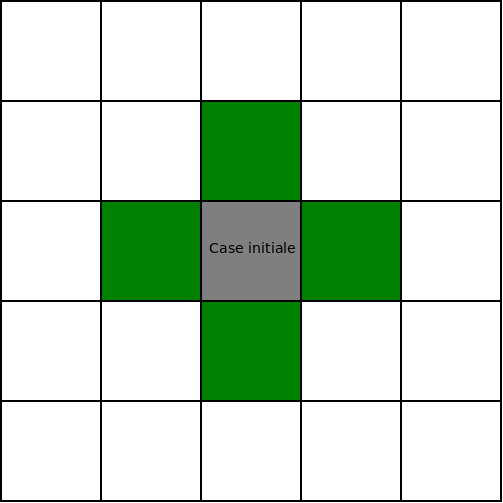
\includegraphics[width=2in]{./schemas/near_attack.png}
  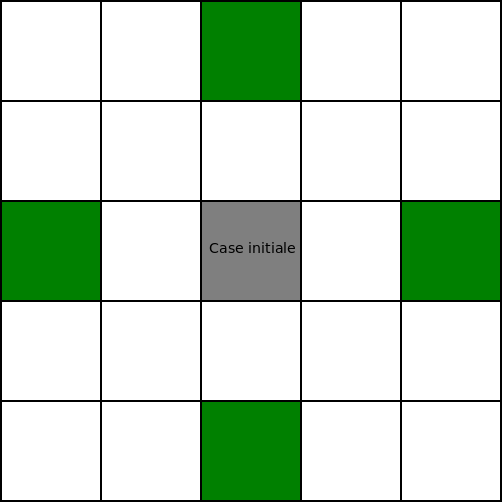
\includegraphics[width=2in]{./schemas/long_attack.png}
  \caption{Cases accessibles (vertes) en fonction du mode d'attaque (rapprochée et à distance)}
  \label{fig:attack}
\end{figure}

\paragraph{}
Une attaque \textbf{rapprochée} se déroule de la façon suivante :

\begin{enumerate}
  \item L'unité ayant le plus de points de défense sur la case ciblée est choisie pour défendre sa case
  \item Le rapport de force entre les points d'attaque de l'attaquant, et les points de défense du défenseur permet de déterminer le gagnant du combat via un tirage aléatoire
  \item Le perdant du combat perd un nombre aléatoire de points de vie, supérieur ou égal à 1
  \item Si le défenseur n'a plus de points de vie et qu'il n'y a aucune autre unité sur la case cible, l'attaquant se déplace automatiquement sur la case cible sans dépenser un point de mouvement supplémentaire
\end{enumerate}

\paragraph{}
Une attaque \textbf{à distance} se déroule d'une autre façon :

\begin{enumerate}
  \item Une unité présente sur la case cible est choisie aléatoirement
  \item Cette unité perd automatiquement un nombre de points de vie aléatoire, supérieur ou égal à 0. On considère en effet que cette unité n'est pas en mesure de se défendre contre l'attaque à distance.
  \item L'unité attaquante ne se déplace en aucun cas à l'issue de l'attaque
\end{enumerate}

